% !TEX root = ../main.tex
% fix page break in toc
% \addtocontents{toc}{\protect\newpage}
\chapter{Results}
  For the purposes of the femtoscopic analysis, events were generated using \verb|THERMINATOR| model for eight different sets of initial conditions corresponding the following centrality ranges: 0-5\%, 0-10\%, 10-20\%, 20-30\%, 30-40\%, 40-50\%, 50-60\% and 60-70\% for the Pb-Pb collisions at the centre of mass energy $\sqrt{s_{NN}} = 2.76$~TeV.
  %
  % ========
  \section{Identical particles correlations}
  % ========
    The correlation functions were calculated separately for the following different pairs of identical particles: $\pi$-$\pi$, $K$-$K$ and  $p$-$p$ for nine $k_T$ bins (in GeV/c): 0.1-0.2, 0.2-0.3, 0.3-0.4, 0.4-0.5, 0.6-0.7, 0.7-0.8, 0.8-1.0 and 1.0-1.2.
    In case of kaons, $k_T$ ranges start from 0.3 and for pions from 0.4 and for both of them the maximum value is 1.0.
    The $k_T$ ranges for the heavier particles were limited to maintain sufficient multiplicity to perform reliable calculations.
    %
    % ========
    \subsection{Spherical harmonics components}
    % ========
      \begin{figure}[h]
        \centering
        \centerline{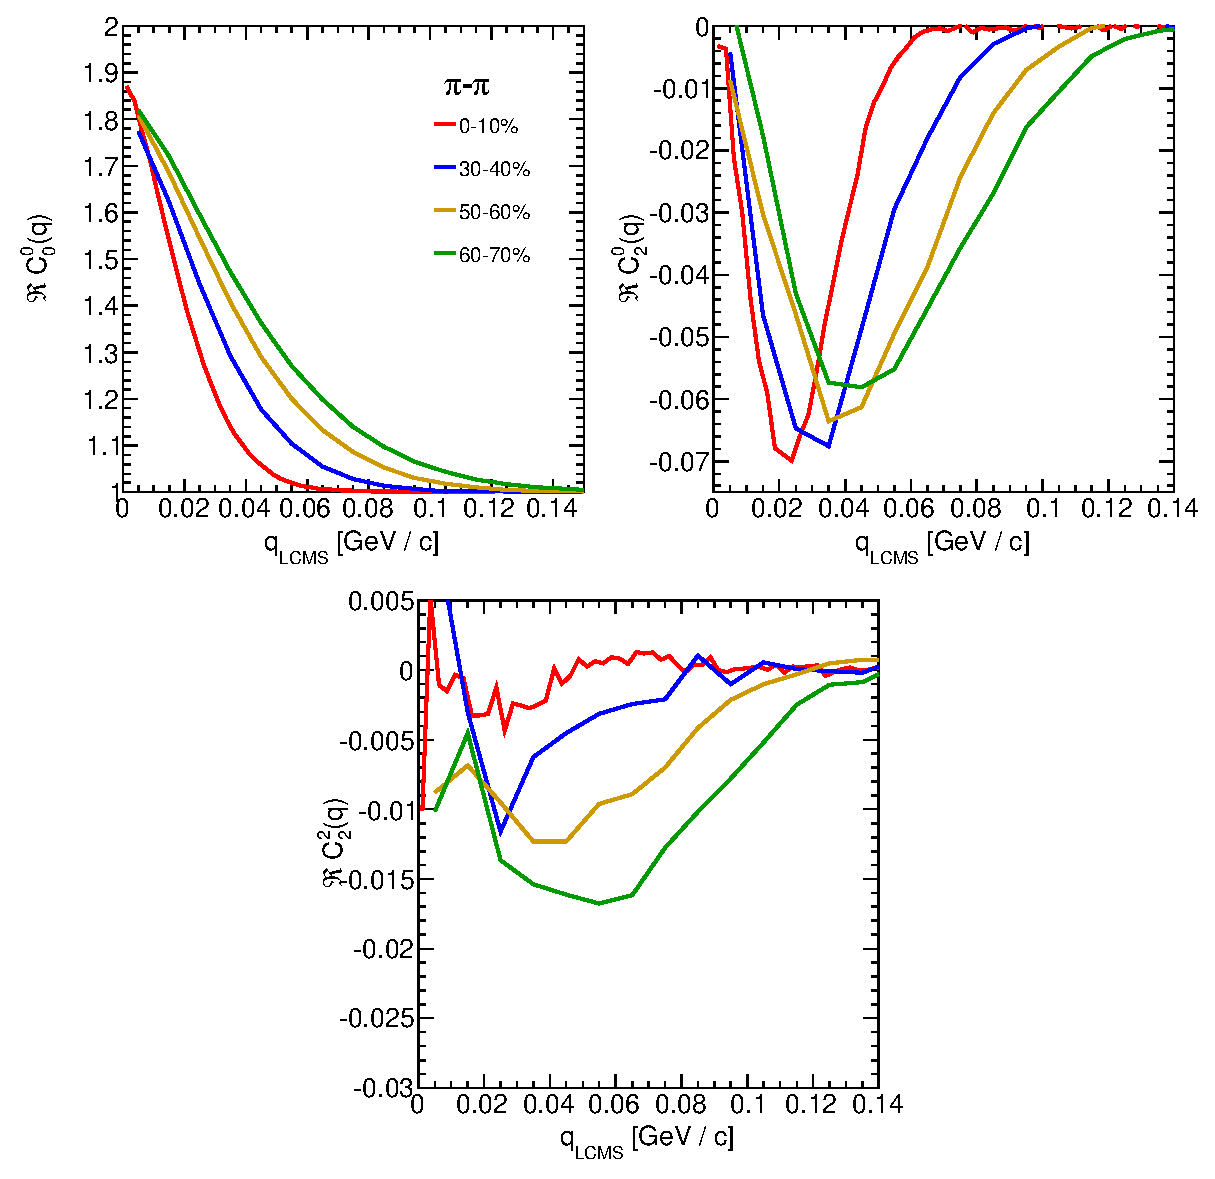
\includegraphics[width=1.0\textwidth]{results/cf3dpi}}
        \caption{no caption}
      \label{fig:cf3dpi}
      \end{figure}

      \begin{figure}[h]
        \centering
        \centerline{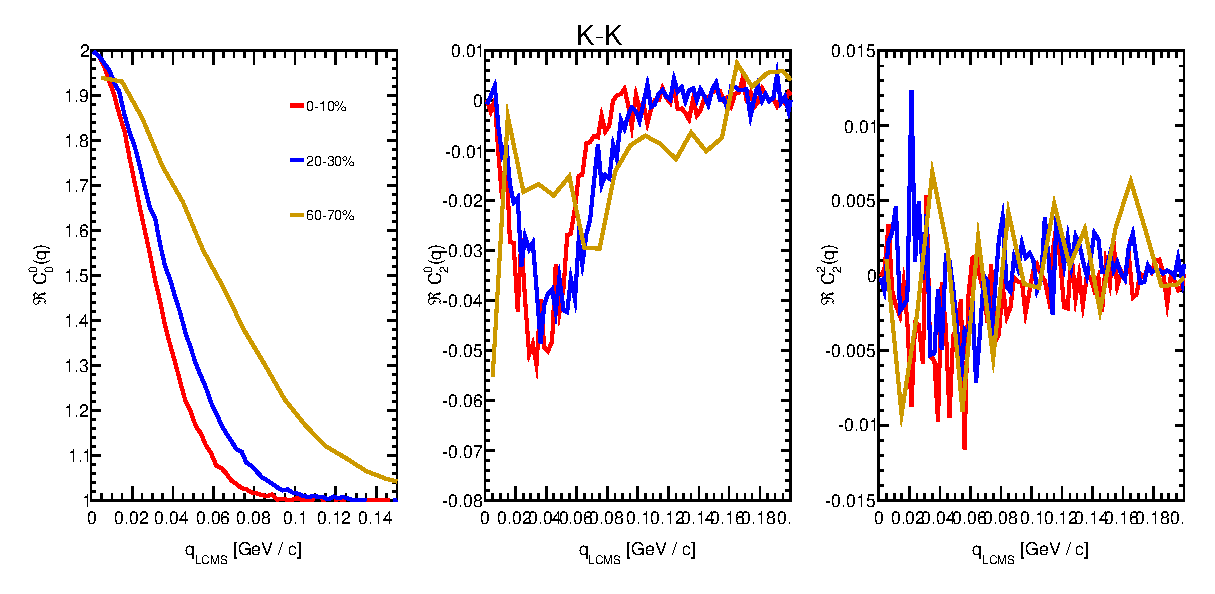
\includegraphics[width=1.0\textwidth]{results/cf3dk}}
        \caption{no caption}
      \label{fig:cf3dk}
      \end{figure} 

      \begin{figure}[h]
        \centering
        \centerline{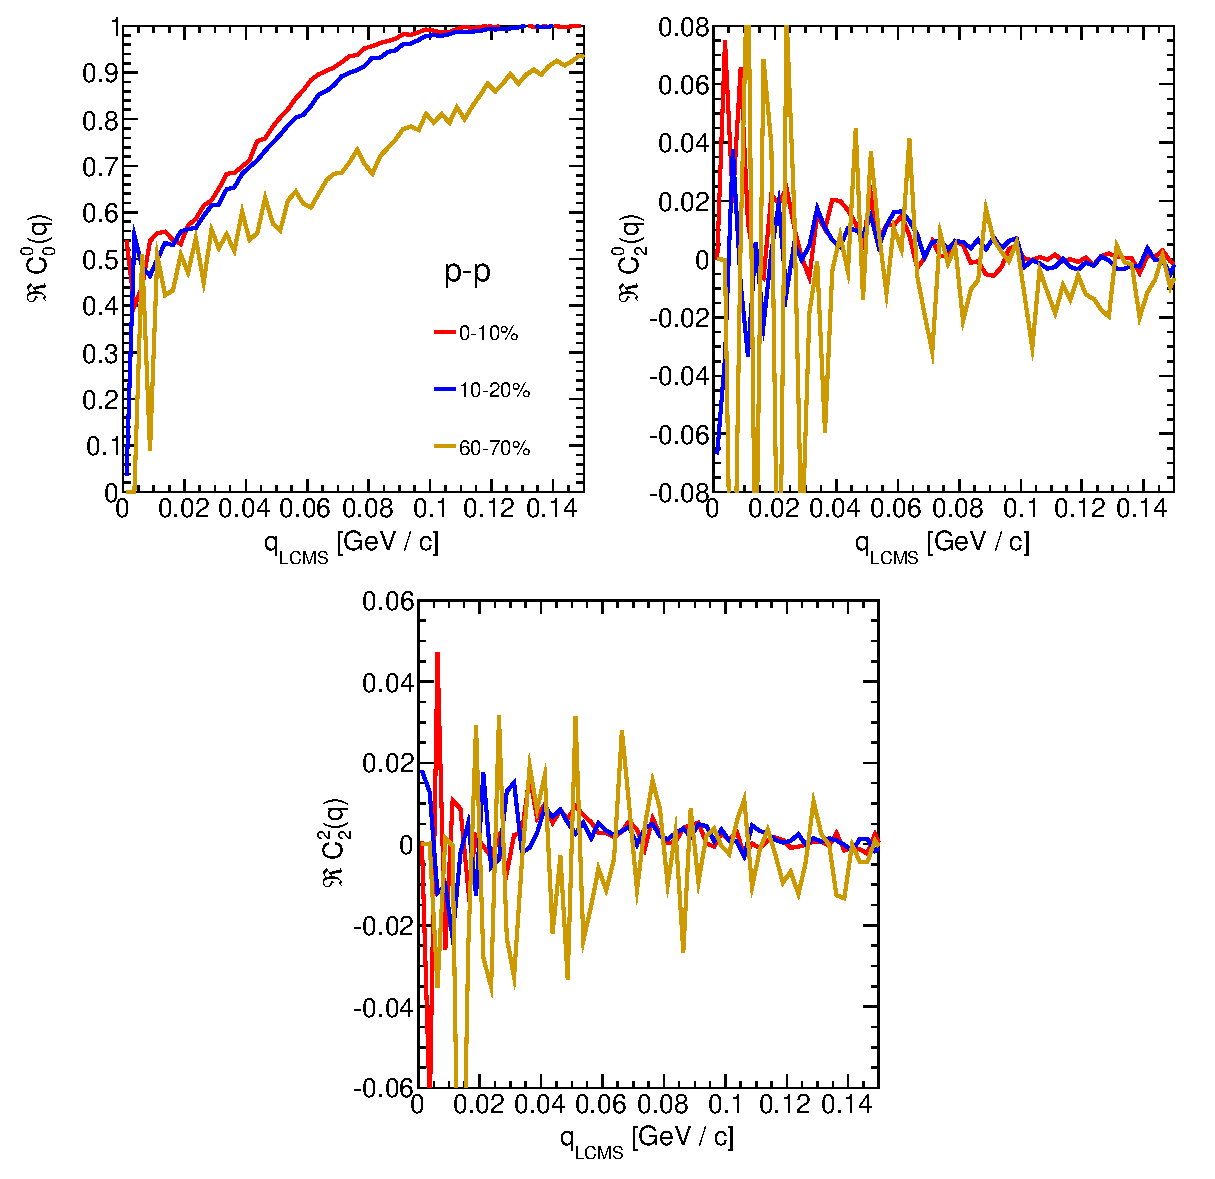
\includegraphics[width=1.0\textwidth]{results/cf3dp}}
        \caption{no caption}
      \label{fig:cf3dp}
      \end{figure}

      foo bar foo bar foo bar foo bar
    \FloatBarrier
    %
    % ========
    \subsection{Centrality dependence of a correlation function}
    % ========
    % napisac o singletowym bozonow i trypletowym protonow
    % pokazac poszerzenie CF vs k_T oraz vs centralnosc
      \begin{figure}[h]
        \centering
        \centerline{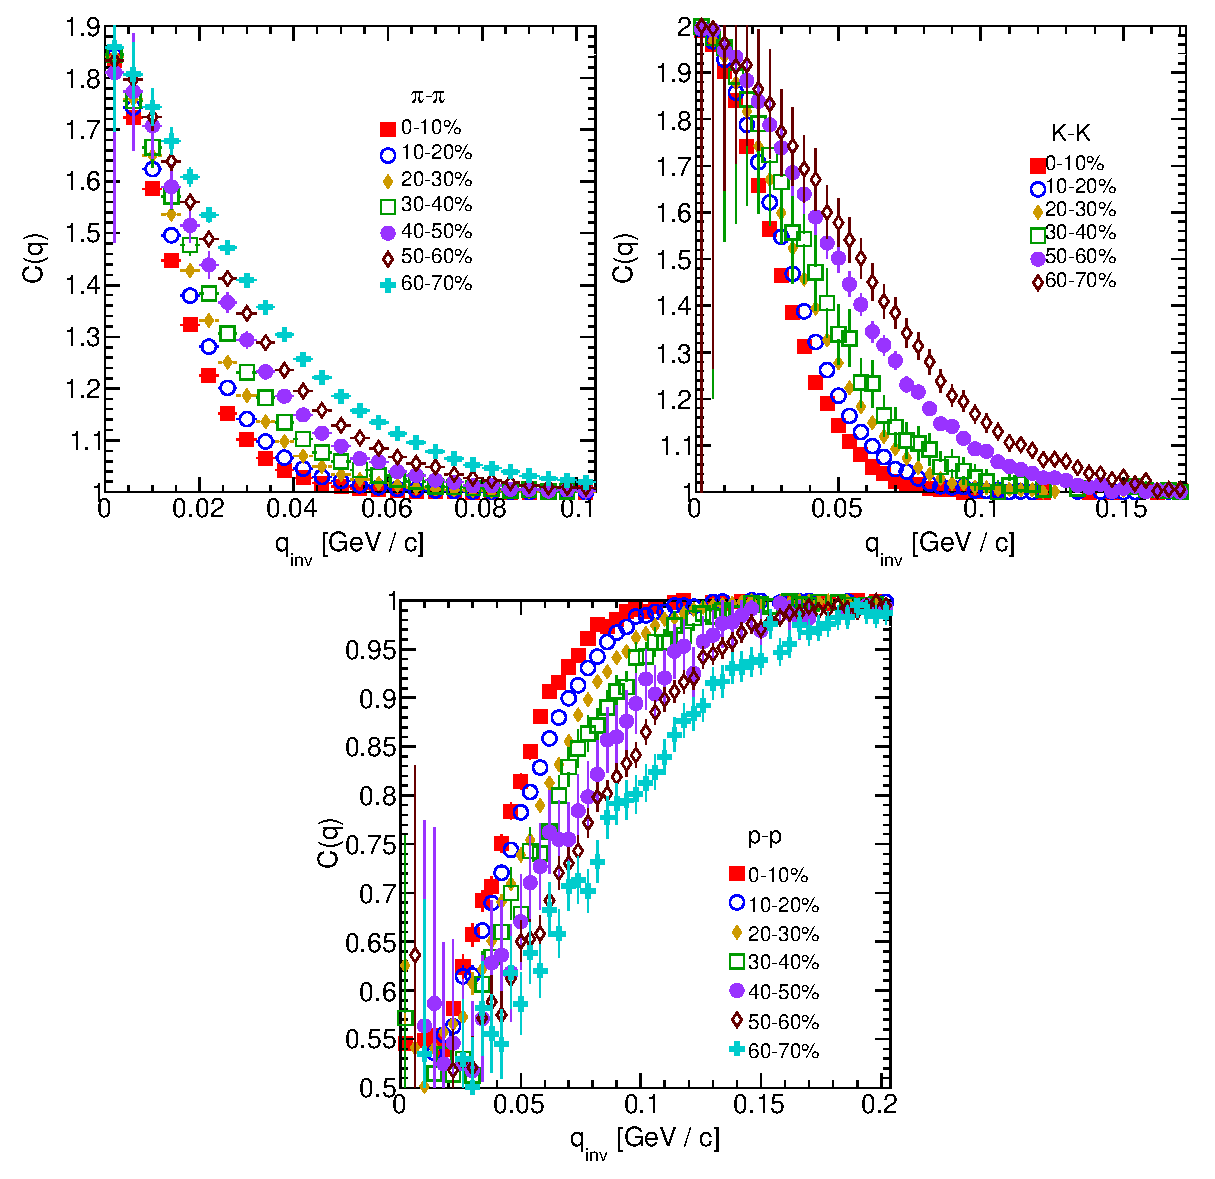
\includegraphics[width=1.0\textwidth]{results/cfvsctr}}
        \caption{no caption}
      \label{fig:centr_dep}
      \end{figure}
    \FloatBarrier
    %
    % ========
    \subsection{$k_T$ dependence of a correlation function}
    % ========
      \begin{figure}[h]
        \centering
        \centerline{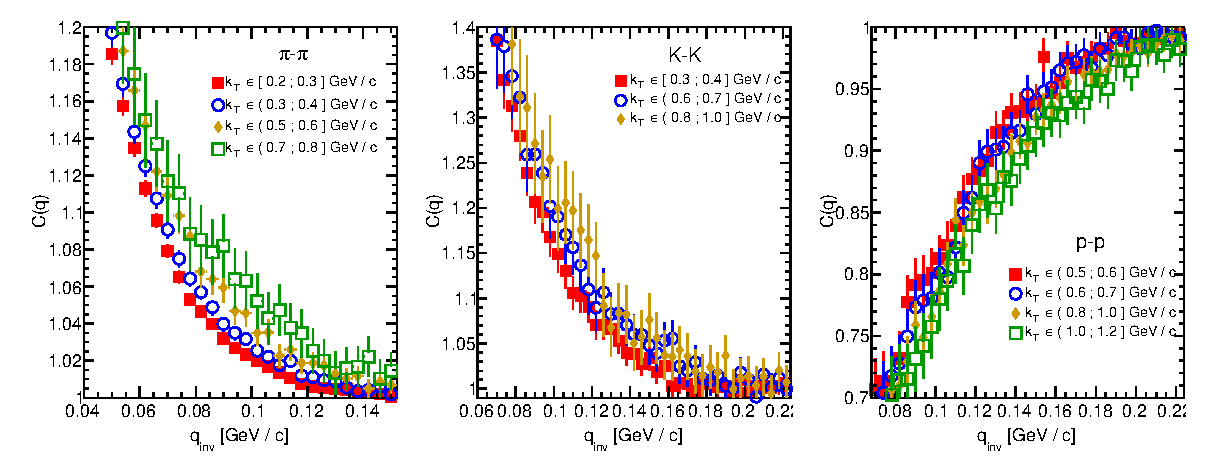
\includegraphics[width=1.0\textwidth]{results/cfvskt}}
        \caption{no caption}
      \label{fig:kt_dep}
      \end{figure}
    \FloatBarrier
  %
  % ========
  \section{Results of the fitting procedure}
  % ========
    %
    % ========
    \subsection{Femtoscopic radii scaling with the transverse mass}
    % ========
      \begin{figure}[h]
        \centering
        \centerline{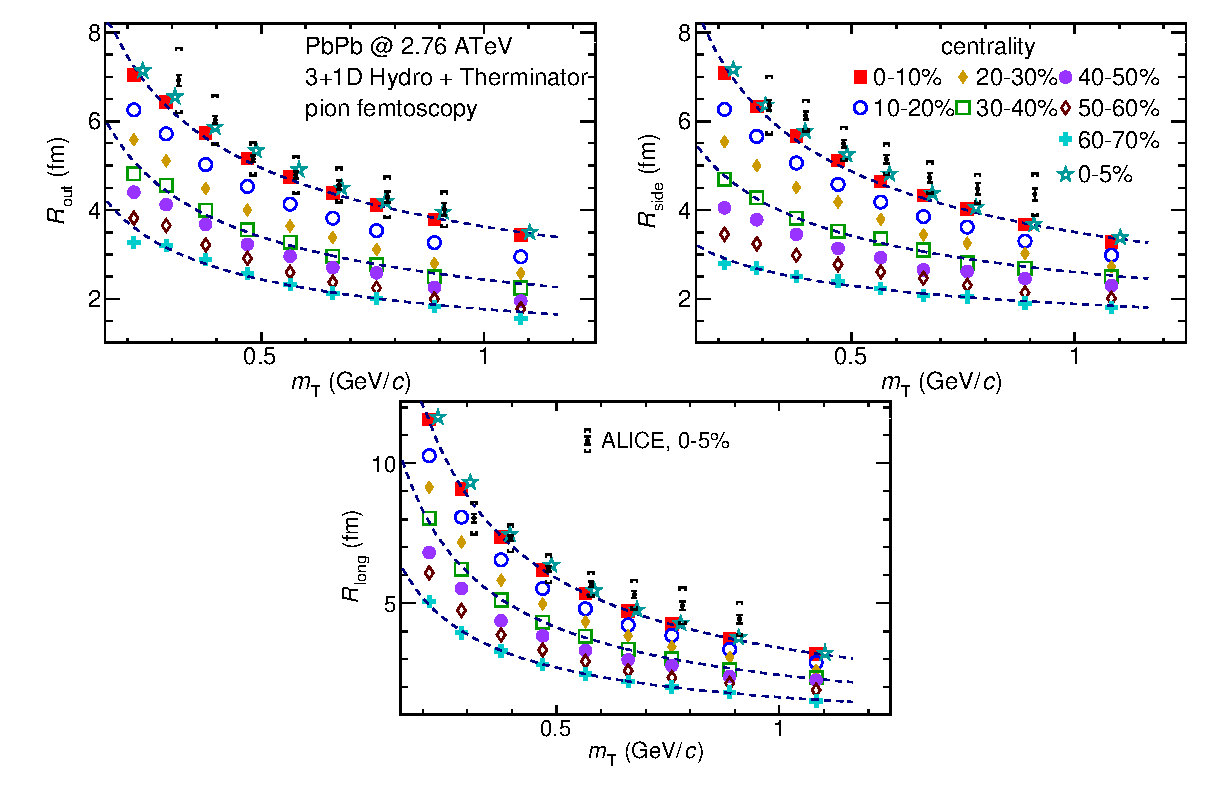
\includegraphics[width=1.05\textwidth]{results/piradii}}
        \caption{no caption~\cite{alice_pion}~\cite{galazyn}.}
      \label{fig:piradii}
      \end{figure}



      \begin{figure}[h]
        \centering
        \centerline{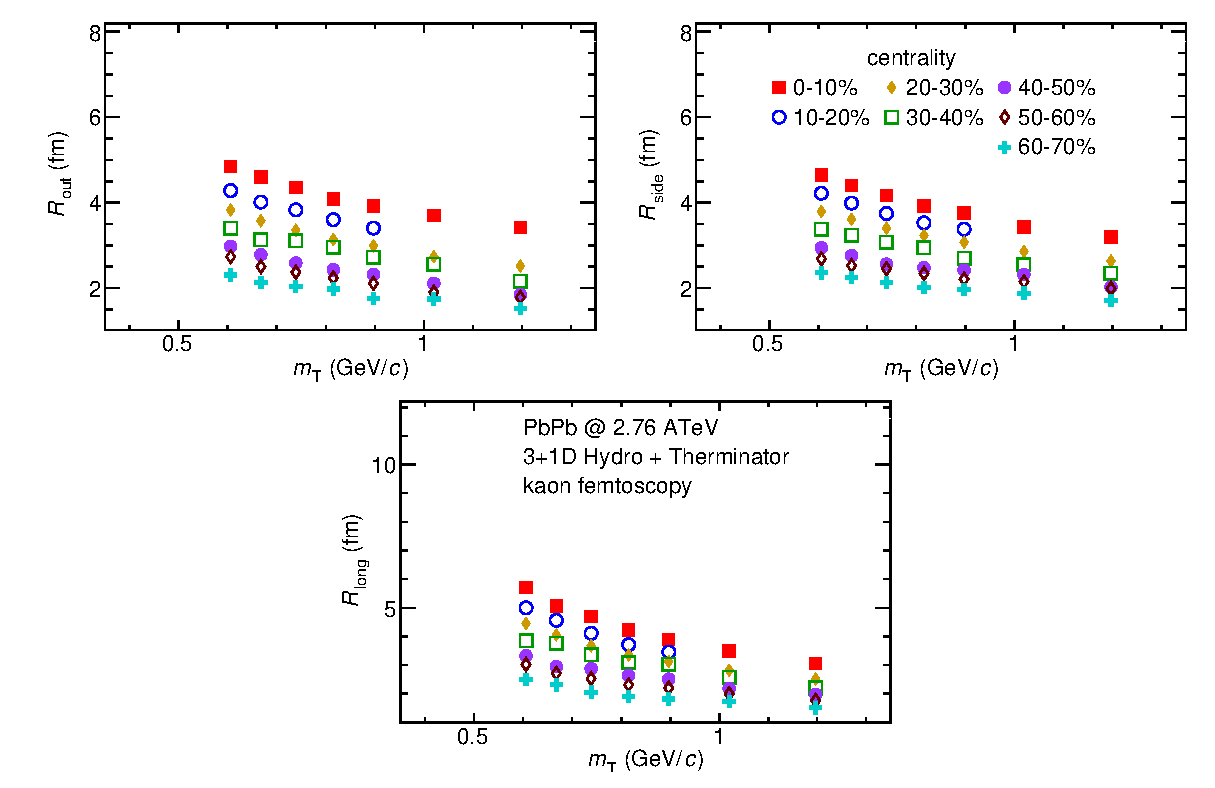
\includegraphics[width=1.05\textwidth]{results/kradii}}
        \caption{no caption~\cite{galazyn}.}
      \label{fig:kradii}
      \end{figure}



      \begin{figure}[h]
        \centering
        \centerline{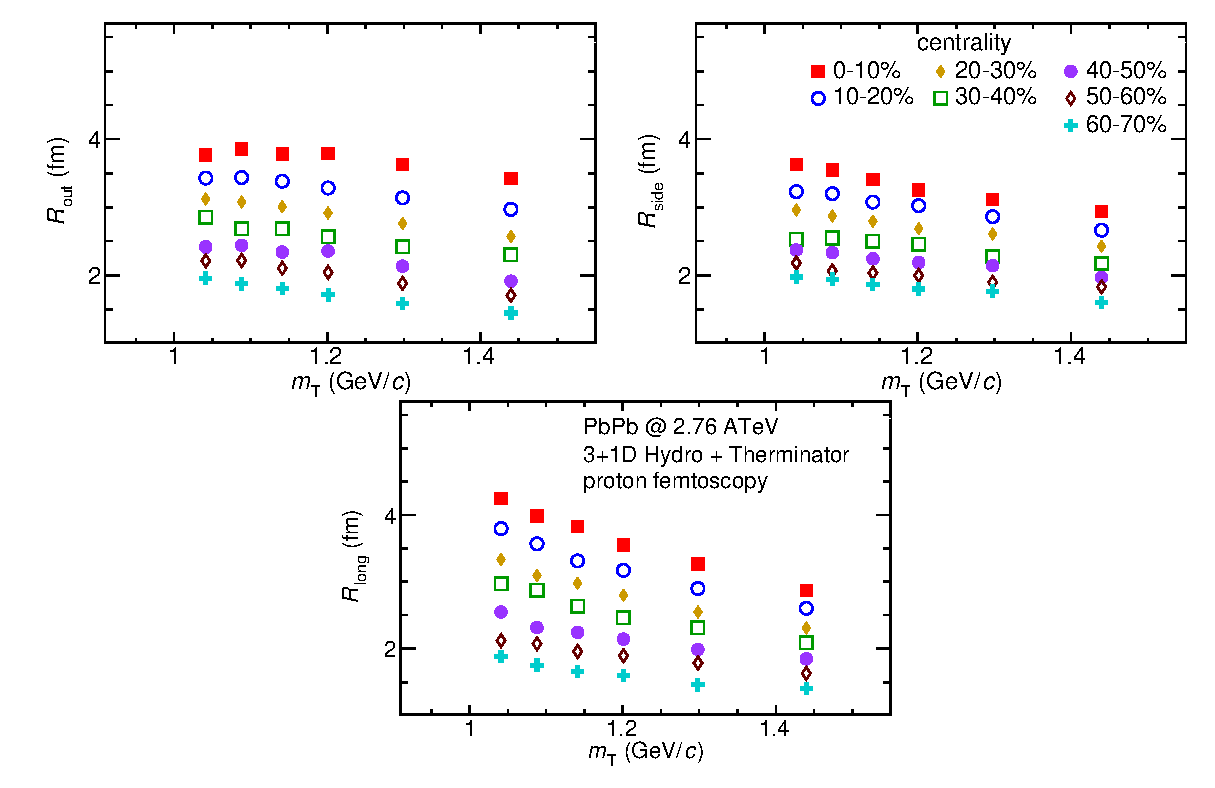
\includegraphics[width=1.05\textwidth]{results/pradii}}
        \caption{no caption~\cite{galazyn}.}
      \label{fig:pradii}
      \end{figure}    

      \begin{figure}[h]
        \centering
        \centerline{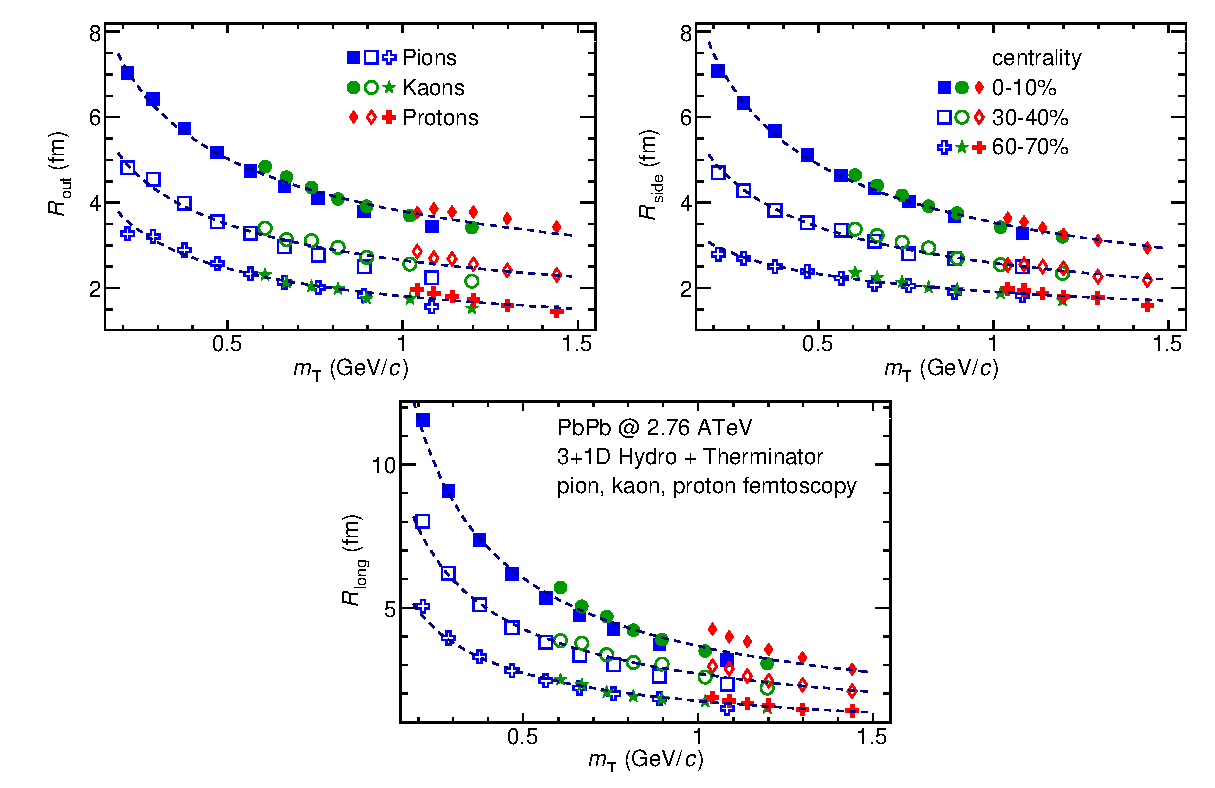
\includegraphics[width=1.05\textwidth]{results/allradii_lcms}}
        \caption{no caption~\cite{galazyn}.}
      \label{fig:allradii}
      \end{figure}    

      \begin{figure}[h]
        \centering
        \centerline{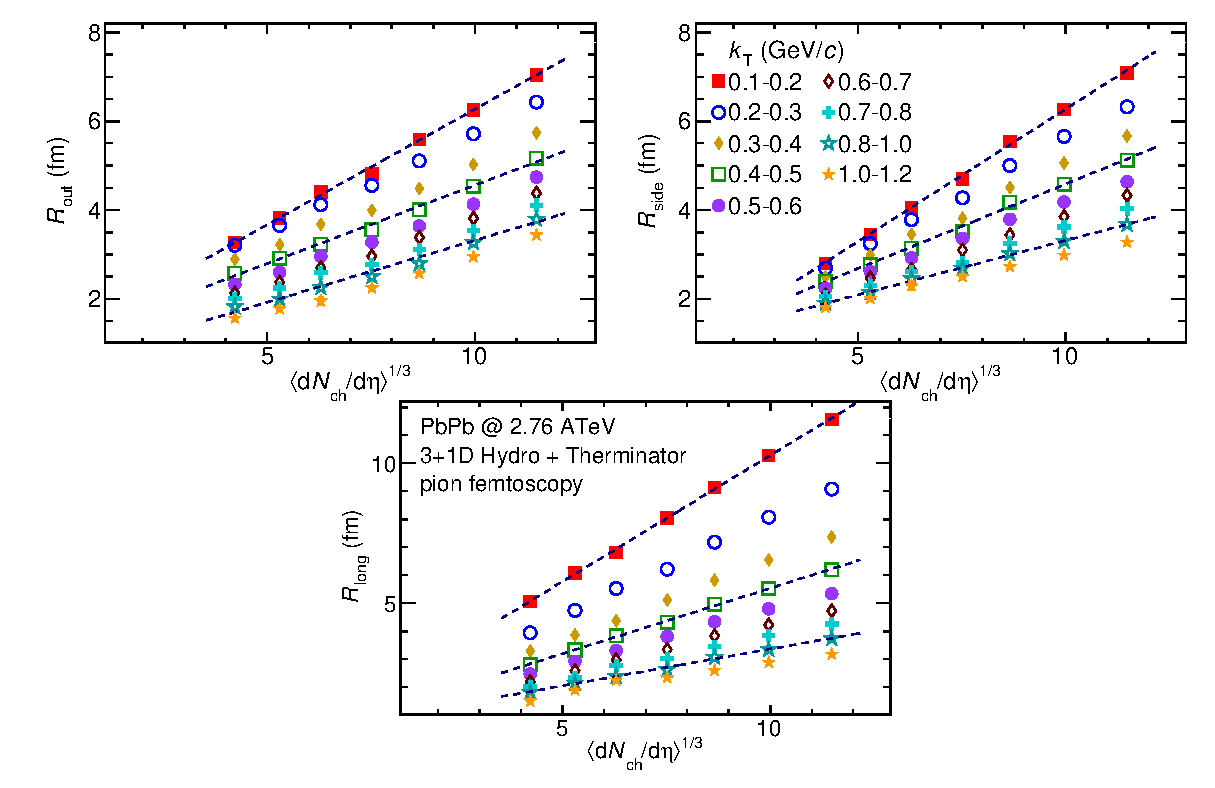
\includegraphics[width=1.05\textwidth]{results/piradii_vs_nch}}
        \caption{no caption~\cite{galazyn}.}
      \label{fig:piradii}
      \end{figure}    

      \begin{figure}[h]
        \centering
        \centerline{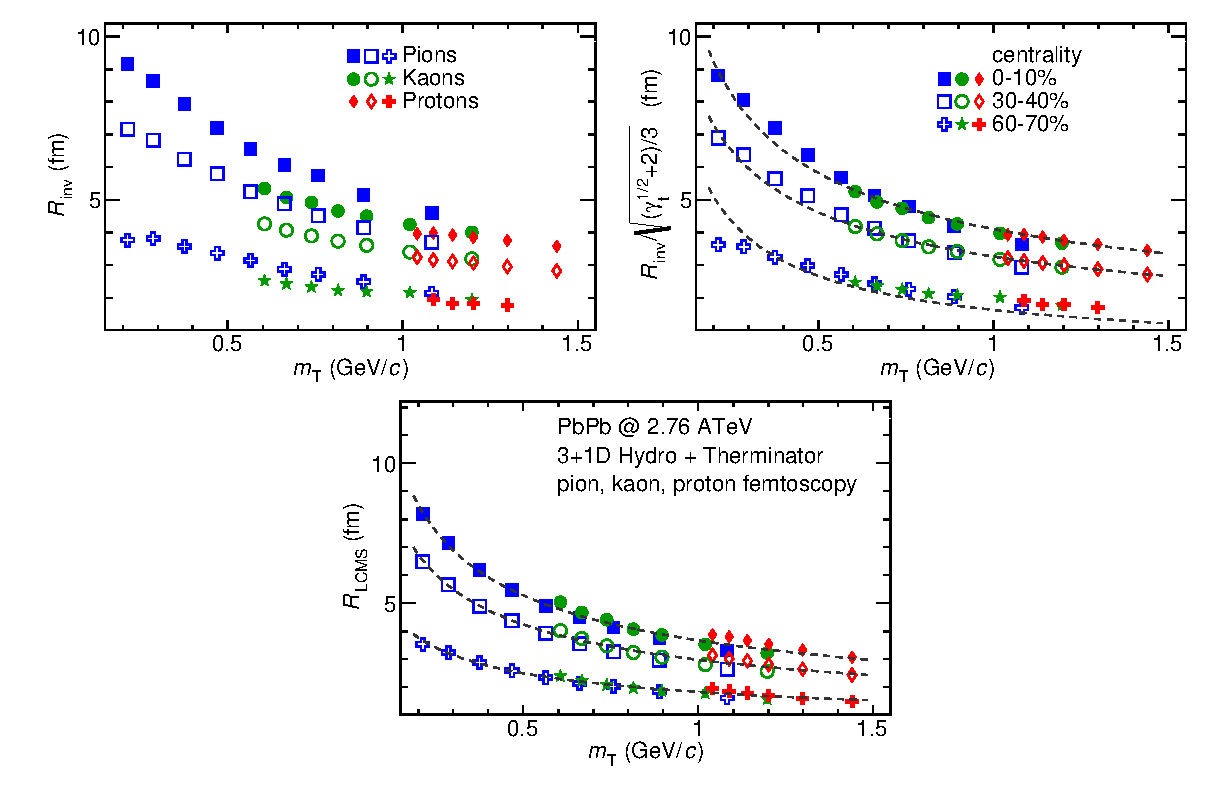
\includegraphics[width=1.05\textwidth]{results/scaling_test}}
        \caption{no caption~\cite{galazyn}.}
      \label{fig:piradii}
      \end{figure}    

      \begin{figure}[h]
        \centering
        \centerline{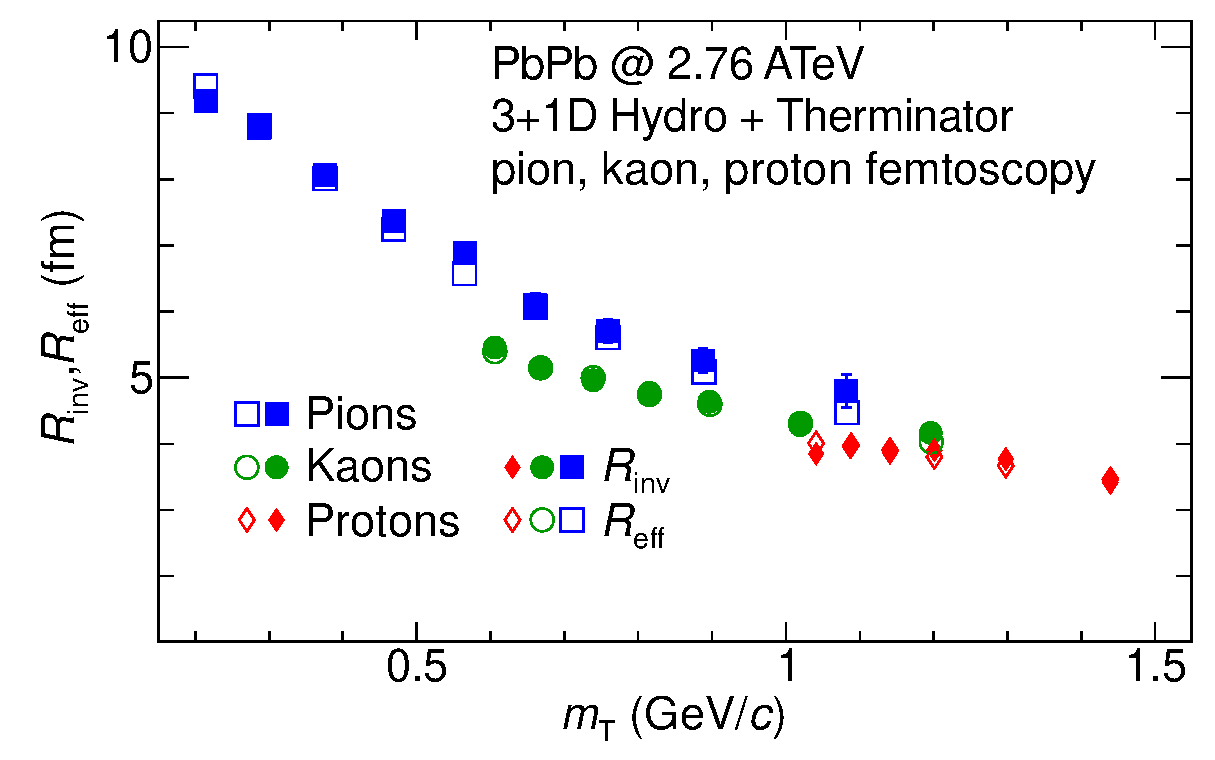
\includegraphics[width=0.55\textwidth]{results/rinvreff}}
        \caption{no caption~\cite{galazyn}.}
      \label{fig:piradii}
      \end{figure}

    \FloatBarrier
  %
  % ========
  \section{Discussion of results}
  % ========

  %% nawiazanie do pracy sinyukova, karpenki,  o złamanym skalowaniu mt w przypadku rescatteringu
